\documentclass[11pt,a4paper]{article}

\usepackage{style2017}
\usepackage{hyperref}

\hypersetup{
    colorlinks =false,
    linkcolor=blue,
   linkbordercolor = 1 0 0
}
\newcounter{numexo}
\setcellgapes{1pt}

\begin{document}



\begin{NSI}
{Exercice}{La récursivité}
\end{NSI}

\addtocounter{numexo}{1}
\subsection*{\Large Exercice \thenumexo}
On donne la fonction suivante:
\begin{center}
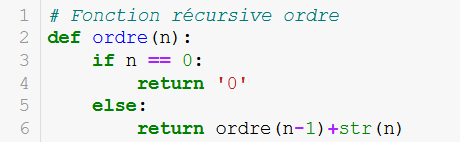
\includegraphics[scale=0.8]{img/ordre.png}
\end{center}
\begin{enumerate}
\item Expliquer pourquoi la fonction \textbf{ordre} est récursive.
\item Que renvoie l'appel \textbf{ordre(4)}?
\item Que se passe-t-il si on change la dernière instruction par \textbf{return str(n)+ordre(n-1)}?
\end{enumerate}

\addtocounter{numexo}{1}
\subsection*{\Large Exercice \thenumexo}
On donne la fonction suivante:
\begin{center}
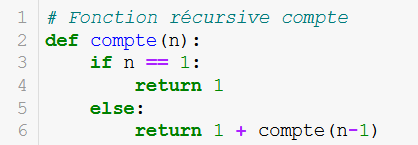
\includegraphics[scale=0.8]{img/compte.png}
\end{center}
\begin{enumerate}
\item Expliquer pourquoi la fonction \textbf{compte} est récursive.
\item Que renvoie l'appel \textbf{compte(5)}?
\item Que se passe-t-il si on change la dernière instruction par \textbf{return 1+compte(n-2)}?
\end{enumerate}

\addtocounter{numexo}{1}
\subsection*{\Large Exercice \thenumexo}
On donne le script suivant et la table de caractères ASCII:
\begin{center}
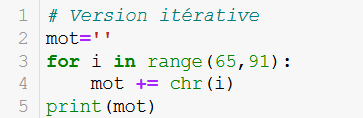
\includegraphics[scale=0.8]{img/alphabet.png}
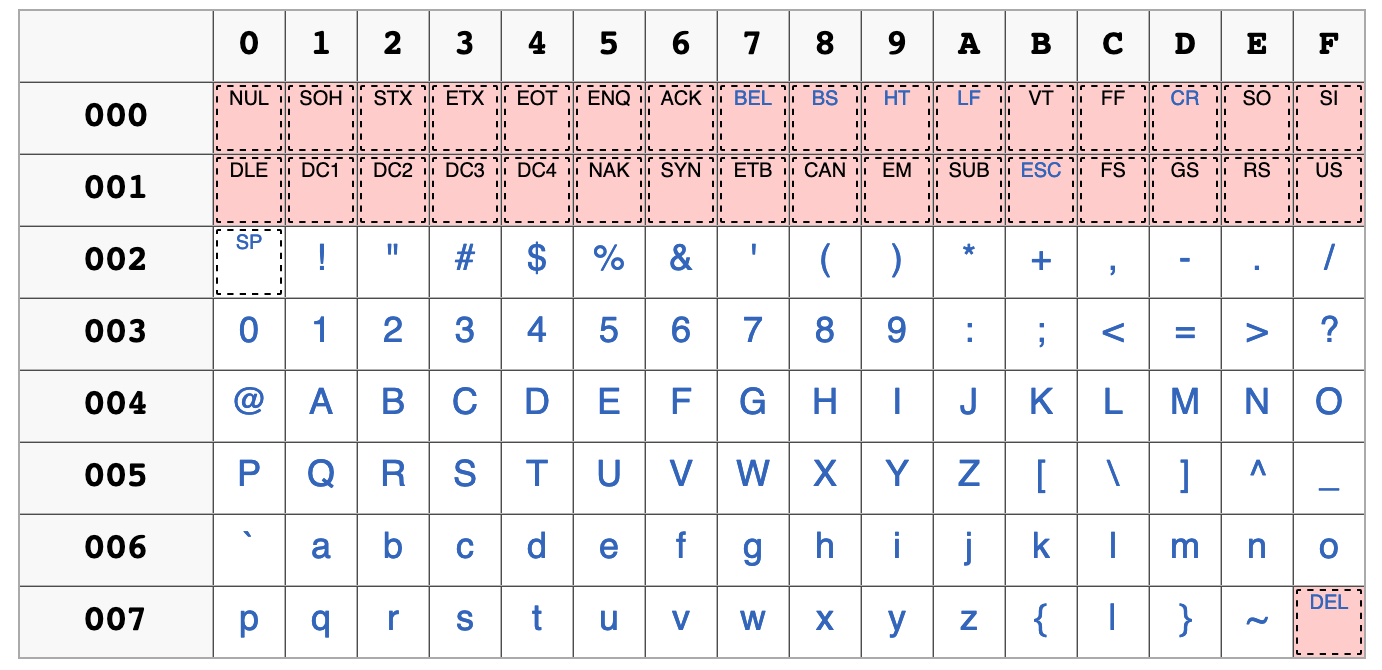
\includegraphics[scale=0.4]{img/tableASCII.png}
\end{center}

On rappelle que la fonction Python \textbf{chr} prend en argument un nombre entier N en écriture décimale et renvoie le caractère ASCII associé.

\begin{enumerate}
\item Quelle est la valeur renvoyée par la commande \textbf{chr(65)} ? Justifier.
\item Quel est l'affichage à l'issu du script ?
\item Écrire la fonction récursive \textbf{affiche\_recursif} renvoyant le même résultat que le script ci-dessus.
\end{enumerate}

\addtocounter{numexo}{1}
\subsection*{\Large Exercice \thenumexo}
Lorsqu'on effectue une remise de 10\% sur un prix, cela revient à multiplier ce prix par la valeur $1-10/100$.

On veut calculer des baisses successives de 10\% sur une valeur, le nombre de remises étant défini à l'avance.
\begin{enumerate}
\item Calculer trois remises successives de 10\% sur un prix de 100 \euro.
\item Montrer en détaillant le calcul qu'un algorithme récursif peut s'appliquer.
\item Écrire un script itératif qui calcule $n$ remises successives de 10\% sur un prix. On utilisera les variables \textbf{prix} et \textbf{n}. La variable \textbf{prix} contiendra la valeur finale.
\item Vérifier votre script avec un prix de 100 pour $n=3$ remises.
\item Écrire la fonction récursive \textbf{remise\_successive} qui calcule $n$ remise de 10\% sur un prix défini à l'avance.
\end{enumerate}



\addtocounter{numexo}{1}
\subsection*{\Large Exercice \thenumexo}
En mathématiques, pour trouver le plus grand commun diviseur de 2 nombres entiers, on applique l'algorithme d'Euclide, donné ci-dessous en python:
\begin{center}
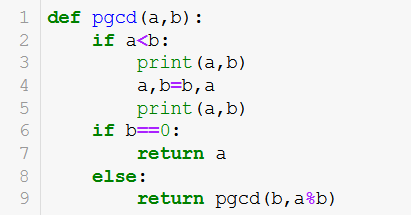
\includegraphics[scale=0.8]{img/ex-pgcd.png}
\end{center}

\begin{enumerate}
\item S'agit-il d'une fonction récursive ? Pourquoi ?
\item \begin{enumerate}
\item Que calcule l'opération $a\%b$ dans la dernière ligne de la fonction ?
\item Quelle est la valeur de $12\%7$ ?
\item Que se passe-t-il si $a$ est strictement inférieur à $b$ ?
\end{enumerate} 
\item Quelle est la signification des instructions aux lignes 2 et 3 de la fonction ?
\item Donner les différentes phases d'exécution de l'appel $\text{pgcd}(28,42)$
\end{enumerate} 

\addtocounter{numexo}{1}
\subsection*{\Large Exercice \thenumexo}

\begin{enumerate}
\item Calculer :
\begin{tabular}{*{4}{L{3.5cm}}}
\textbf{a)} $1 \times 2$ &\textbf{b)} $1 \times 2 \times 3$ & \textbf{c)} $1 \times 2 \times 3 \times 4$ & \textbf{d)} $1 \times 2 \times 3 \times 4 \times 5$ \\
\end{tabular}
\item Les produits précédents s'appellent \textbf{factorielles} et se notent en mathématiques avec un point d'exclamation.

Par exemple : $\text{factorielle(4)}=1 \times 2 \times 3 \times 4 = 4!$
\begin{enumerate}
\item Quelle est la valeur de $\text{factorielle(1)}$ ?
\item Quelle égalité peut-on écrire entre $\text{factorielle(4)}$ et $\text{factorielle(5)}$?
\item Pour tout nombre entier $n$, exprimer $\text{factorielle($n$)}$ en fonction de $n-1$.
\end{enumerate}  
\item Écrire la fonction récursive \textbf{factorielle(n)} qui prend en paramètre un nombre entier $n$ et renvoie la valeur de sa factorielle. On donne ci-dessous le squelette de la fonction.
\begin{center}
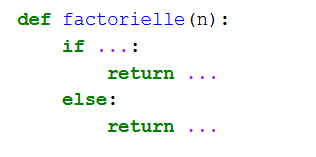
\includegraphics[scale=0.8]{img/factorielle_vide.png}
\end{center}

\end{enumerate}

\addtocounter{numexo}{1}
\subsection*{\Large Exercice \thenumexo}
\begin{enumerate}
\item Écrire une fonction récursive \textbf{puissance} qui prend en paramètres un flottant $x$ non nul et un entier naturel $n$ et qui renvoie $x^{n}$. On se base sur la définition mathématique : $x^{0}=1$ et $x^{n}=x \times x^{n-1}$.
\item On propose une seconde méthode de calcul de la puissance. 

Pour cela, on note $x^{0}=1$ et on remarque que si $n=2k$ (n pair), alors $x^{n}=(x^{2})^{k}$ et si $n=2k+1$ (n impair) alors $x^{n}=x^{2k+1}=x(x^{2})^{k}$.

Écrire une fonction récursive utilisant cette méthode de calcul.
\end{enumerate}


\addtocounter{numexo}{1}
\subsection*{\Large Exercice \thenumexo}
\begin{enumerate}
\item Expliquer quel est le résultat renvoyé par le code suivant:
\begin{center}
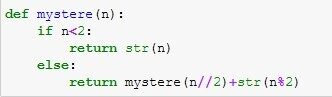
\includegraphics[scale=0.8]{img/ex-mystere.eps}
\end{center}
\item Écrire une fonction binaire qui prend en paramètres un entier relatif $r$ et un entier naturel $n$ strictement positif, et qui renvoie la représentation en machine de $r$ sur $n$ bits. La méthode utilisée est celle du complément à $2$.

Déterminer l'écriture binaire sur $n$ bits d'un nombre négatif $r$ revient à déterminer l'écriture binaire du nombre positif  $r+2^{n}$.

Exemple de l'écriture binaire du nombre $-35$ sur 7 bits : $-35+2^{7}=93=1011101_{2}$.
\end{enumerate}


\addtocounter{numexo}{1}
\subsection*{\Large Exercice \thenumexo}
\begin{enumerate}
\item Dans un idle (pyzo, thonny, python) saisir le programme ci-dessous et le tester:
\begin{center}
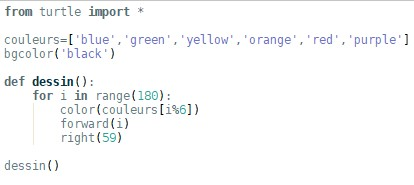
\includegraphics[scale=0.8]{img/pgm-dessin-spirale.eps}
\end{center}
\item En donner une version récursive.
\end{enumerate}


\addtocounter{numexo}{1}
\subsection*{\Large Exercice \thenumexo}
La fonction \textbf{fibonacci(n)}, qui doit son nom au mathématicien Leonardo Fibonacci, est définie récursivement, pout tout entier $n$, de la manière suivante:
\begin{align*}
\text{fibonnacci}(n)=\left\lbrace \begin{array}{ll}
0 & \text{si~} n=0,\\
1 & \text{si~} n=1,\\
\text{fibonnacci}(n-2) + \text{fibonnacci}(n-1) & \text{si~} n>1.\\
\end{array}
\right.
\end{align*}
\begin{enumerate}
\item Calculer fibonacci(5).
\item Écrire en python cette fonction fibonacci.
\end{enumerate}


\end{document}
